\centering
% for double arrows a la chef
% adapt line thickness and line width, if needed
\begin{tikzpicture}[thick]
\node[] (start) {};
 \node[draw,circle,minimum size=1.5cm,left = 0.5cm of start] (f) {f$_{\text{compute}}$};
 \node[draw,right = 0.5cm of start,circle,minimum size=1.5cm] (K) {$\kse
\midtheta$};
 %\node[below left of=f_K,xshift=-1.7cm,yshift=-0.1cm] (theta) {$\bm{\theta} \sim P(\bm{\theta})$};
 \node[draw,rectangle,below=1.2cm of start, text width = 8cm] (gpmem) {\centering\texttt{gpmem}\vspace{2mm}

\small$\text{memo table} = (\xbf,\ybf)$\vspace{1mm}

\small$\;\;\;\;\;\;\;\;\;\;P(f_{emu}(x) \mid \xbf,\ybf,\thetabf)\sim
\mathcal{N}\big(\mupost,\Kpost)\big)$
 };
%  \node[draw,rectangle,color=ForestGreen,below = .1ex of gpmem,minimum width=1.5cm, minimum height=0.4cm,yshift=0.9cm,xshift=0.3cm] (mark) {};
  \node[draw,rectangle,dashed,right=2cm of K, text width = 3.5cm] (math) {\footnotesize
 $\kse\,= \sigma^2 \exp(-\frac{(x-x^\prime)^2}{2\ell^2})$\vspace{1mm}

 $\thetabf \;\;\,\,= \{\sigma,\ell \} \rightarrow$ Scope\vspace{1mm}

 $\sigma\;\;\; \sim P(\sigma)\, \rightarrow$ Block 0\vspace{1mm}

 $\ell\;\;\;\, \sim P(\ell)\;\, \rightarrow$ Block 1\vspace{1mm}


%\scriptnotesize
%
%%$\mu(\mathbf{x}) =\mu(\mathbf{x}) + \mathbf{K}_\theta(\mathbf{x},\mathbf{x}_{past})\mathbf{K}_\theta(\mathbf{x}_{past},\mathbf{x}_{past})^{-1}(\mathbf{y}_{past} - \mu(\mathbf{x}_{past}))$
 };
 \node[draw,rectangle,dashed,minimum size=1cm,left= 2.2cm of f] (resources) {
\includegraphics[width=2.8cm]{figs/resources.png}};

\node[draw,rectangle,below=0.8cm of gpmem,text width =7cm] (f_emu) {\centering $f_{emu}$ \vspace{1mm}

\begin{tabular}{l|l}\footnotesize
  \footnotesize$x$ & \footnotesize$f(x)$ \\ \hline
  \footnotesize $x_1$  &\footnotesize$y_1$ \\
 \footnotesize  $x_2$  & \footnotesize$y_2$ \\
 \footnotesize$\cdots$ & \footnotesize $\cdots$
 \end{tabular}
 $\;\;\;\;$
 \begin{tabular}{l}
 \small Parameters:\\
\small  Kernel lengthscale $\ell$  \\
\small Kernel scale-factor $sf$
 \end{tabular}

};
%\node[right = 1.2 cm of f_emu,inner sep = 0pt,outer sep=0pt,minimum size=25pt] (emu_annotate) {Infer: $\theta\;$};

\node[below = .1ex of gpmem,inner sep = 0pt,outer sep=0pt,xshift=-0.3cm] (helper1) {};
\node[below = .1ex of gpmem,inner sep = 0pt,outer sep=0pt,xshift=0.7cm] (helper2) {};

\node[above = .1ex of f_emu,inner sep = 0pt,outer sep=0pt, xshift=0mm] (helper_emu) {};

\node[above = 0.75cm of resources,inner sep = 0pt,outer sep=0pt] (helper_resource_top) {};
\node[left = 1cm of f_emu] (x_hat) {$\xprime$} ;
\node[right = 1cm of f_emu] (GaussianHat)
{$\yprime$} ;

%\node[right =1. cm  of f_emu, yshift=1.5cm] (infer) {\small Infer: $\ell$, $sf$} ;

% 1st pass: draw arrows

  \draw[thick,dashed,->] (resources) --node [pos=0.5,below] {\footnotesize resource}  node [pos=0.5,above] {\footnotesize outside} (f);
  \draw[thick,dashed,->] (math) -- node [pos=0.5,above] {\footnotesize Kernel} (K);
  \draw[thick,->] (K) -- (gpmem);
  \draw[thick,->] (f) -- (gpmem);
 % \draw[thick,->] (theta) -- (gpmem);
  \draw[thick,->] (gpmem) -- (f_emu);

 % \draw[thick,->,color=ForestGreen] (helper_compute) -- node[pos=0.5, sloped, below] {probe} (helper1);
 % \draw[thick,->,color=ForestGreen] (helper2) -- node[pos=0.5, sloped,above] {improves} (helper_emu);
   % \draw[thick,->,dashed,color=ForestGreen] (helper_resource) -- node[pos=0.5,above] {$f_{com}(x_2)=y_2$} (f_compute);
  %  \draw[thick,->,dashed,color=ForestGreen] (helper_resource) -- (resources);
     \draw[thick,->,dashed] (x_hat) -- (f_emu);
     \draw[thick,->,dashed] (f_emu) -- (GaussianHat);
 % \draw[thick,->] (theta) -- (gpmem);


%\path[](f_emu) edge [in=90, out=50,thick] (emu_annotate)
%    (emu_annotate) edge [->,in=310, out=270,thick]  (f_emu);
  % Note: If you have no branches, the 2nd pass is not needed
\node[above=1 cm of start] (alabel) {(a) \gpmem: Schematic};
\end{tikzpicture}


\begin{tabular}{ll}
% line 1
& \\
\hline
\small\begin{lstlisting}[mathescape,escapechar=\#]
define f = proc(x) {
  exp(-0.1*abs(x-2)) * 10 * cos(0.4*x) + 0.2};#\vspace{1mm}#
assume (f_compute, f_emu) = gpmem(f, kse);#\vspace{1mm}#
sample f_emu(array(-20, $\cdots$, 20));

\end{lstlisting}
& \raisebox{-0.5\height}{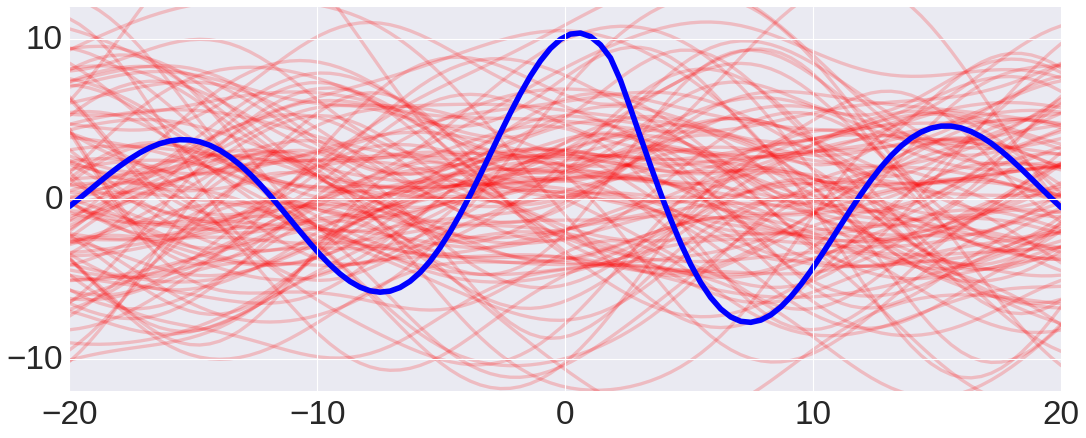
\includegraphics[height=2.0cm]{figs/tutorial_1.png}} \\ \hline
% line 2
\small\begin{lstlisting}[mathescape,escapechar=\#]
predict f_compute(12.6);

sample f_emu(array(-20, $\cdots$, 20));

\end{lstlisting}
 &  \raisebox{-0.5\height}{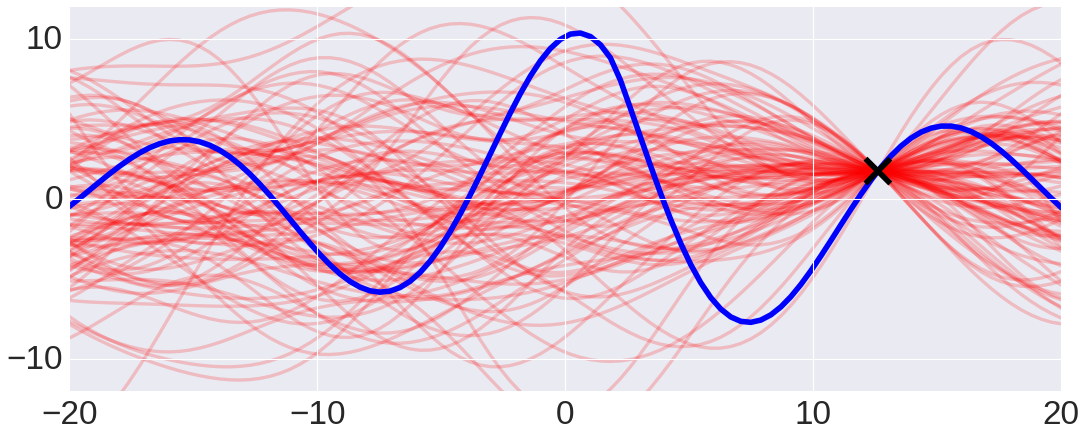
\includegraphics[height=2.0cm]{figs/tutorial_2.png}}  \\ \hline
% line 3
 \small\begin{lstlisting}[mathescape,escapechar=\#]
predict f_compute(-6.4);

sample f_emu(array(-20, $\cdots$, 20));

\end{lstlisting}
 &  \raisebox{-0.5\height}{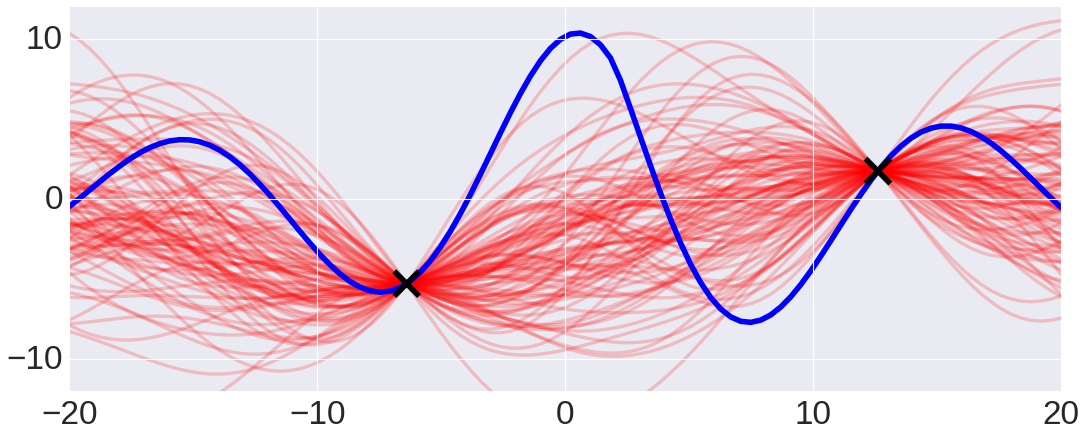
\includegraphics[height=2.0cm]{figs/tutorial_3.png}}  \\ \hline
% line 4
 \small\begin{lstlisting}[mathescape,escapechar=\#]
observe f_emu(-3.1) =  2.60;
observe f_emu(7.8)  = -7.60;
observe f_emu(0.0)  = 10.19;#\vspace{1mm}#
sample f_emu(array(-20, $\cdots$, 20));

\end{lstlisting}
 &   \raisebox{-0.5\height}{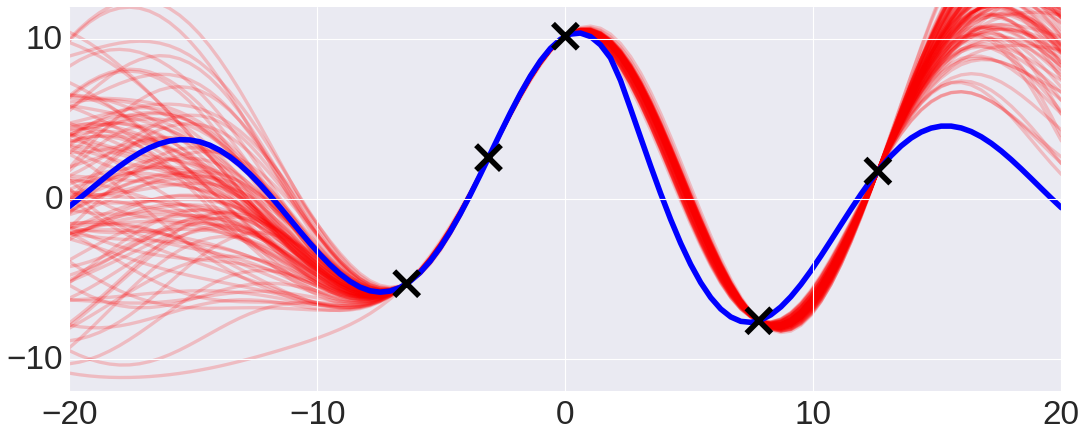
\includegraphics[height=2.0cm]{figs/tutorial_5.png}} \\ \hline
% line 5
 \small\begin{lstlisting}[mathescape,escapechar=\#]
infer mh("hyper_parameter", one, 50);

sample f_emu(array(-20, $\cdots$, 20));

\end{lstlisting}
 &   \raisebox{-0.5\height}{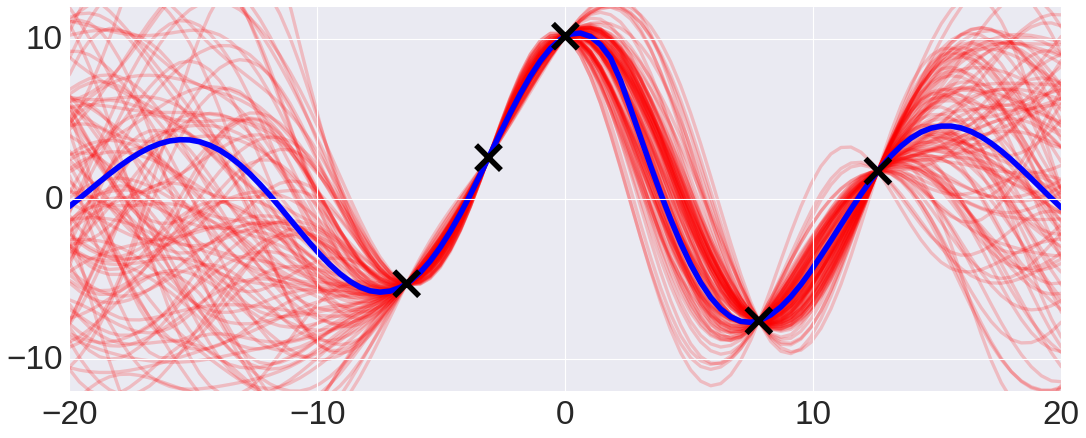
\includegraphics[height=2.0cm]{figs/tutorial_6.png}}
\end{tabular}
